\documentclass[12pt]{article}

\usepackage{fancyhdr}
\usepackage{fullpage}
\usepackage{hyperref}
\usepackage[table]{xcolor}
\usepackage[font=scriptsize]{caption}
\usepackage[pdftex]{graphicx}
\newcommand{\HRule}{\rule{\linewidth}{0.5mm}}
\usepackage[UKenglish]{isodate}% http://ctan.org/pkg/isodate
\usepackage {tabularx}
\usepackage[utf8]{inputenc}
\usepackage[english]{babel}
\usepackage{changepage}% http://ctan.org/pkg/changepage
\usepackage{pdfpages}
\usepackage{enumitem}
\usepackage{tikz}
\usepackage{tikz-uml}
\usetikzlibrary{arrows,shadows,positioning}
\usetikzlibrary{shadows.blur}
\usetikzlibrary{shapes.symbols}
\usepackage{tocloft}
\usepackage{pgf-umlsd}
\usepackage{ifthen}
\usepackage{xstring}
\usepackage{pgfopts}
\usepackage{calc}
\usepackage{babel}
\usepackage{anyfontsize}
\usepackage{geometry}
\pagestyle{fancy}
\usepackage{float}
\usepackage{tabu}
\usepackage{soul}

\usepackage[table]{xcolor}
 \definecolor{lightblue}{rgb}{0.93,0.95,1.0}
 \rowcolors{1}{white}{lightblue}
\usepackage{etoolbox}
\makeatletter
\preto\tabular{\global\rownum=1}
\makeatother

% table padding
\usepackage{array}
\setlength\extrarowheight{4pt} % or whatever amount is appropriate

\headheight = 28pt 
\headsep = 12pt
\cleanlookdateon

% Default Page Header & Footer
\renewcommand{\headrulewidth}{0pt}
\fancyhead[L]{}
\fancyhead[C]{}
\fancyhead[R]{}

\fancyfoot[C]{}
\fancyfoot[R]{\thepage}

% Title Page Header Style
\fancypagestyle{titlestyle}
{
     \fancyhf{}
     % Remove header bar
     \renewcommand{\headrulewidth}{0pt}
     
     \fancyfoot[L]{\large\emph{Group Members:}\\Arron \textsc{Solano}\\Brian \textsc{Howell}\\Daniel \textsc{Carroll}\\Michael \textsc{Danko}}
}

\definecolor{light-gray}{gray}{0.90}
\definecolor{dark-gray}{gray}{.65}

\setlength{\parindent}{1cm} % Default is 15pt.

\pagenumbering{roman}

% Table of Contents Settings
\setcounter{secnumdepth}{3} 
\setcounter{tocdepth}{3}
\cftsetindents{subsubsection}{0.9cm}{1.27cm}

% Table of contents dots
\renewcommand{\cftsecleader}{\cftdotfill{\cftdotsep}}

% Blue Title Cells
\newcommand\BlueCell[1]{%
    \multicolumn{1}{c}{\cellcolor{dark-gray}\textcolor{yellow}{#1}}
}

\begin{document}
  \begin{titlepage}
  \thispagestyle{titlestyle}
  \newgeometry{bottom=7cm}
  \begin{center}

    % Upper part of the page. The '~' is needed because \\
    % only works if a paragraph has started.
    %\includegraphics[width=0.35\textwidth]{eps/logo.eps}~\\[1cm]
    %
\includegraphics[width=90mm]{../../logo/500w.png}
    %\textsc{\LARGE Florida State University}\\[1.5cm]
  {\fontsize{80}{96}\selectfont WalleTx}\\[0.6cm]

    \textsc{\normalsize Software Research Specification}\\[0.5cm]

    % Title
    %\HRule \\[0.4cm]
    { \large \bfseries Prestige Worldwide\\[0.4cm] }

    % \HRule \\[1.5cm]
  %\null
  %\vfill
    % Author and supervisor

    % Bottom of the page

  \end{center}
  \restoregeometry
\end{titlepage}


  \tableofcontents
  %\listoffigures
  \clearpage
  
  % reset page numbering
  \pagenumbering{arabic}
  \setcounter{page}{1}

  \section{Introduction}

	\subsection{Purpose}
	
	Bitcoin WalleTx (WalleTx) is a bitcoin wallet tracker tool for Android that assists users in monitoring their bitcoin balance, transaction history, and spending trends across multiple wallets. It is common for bitcoin users to possess numerous wallets, yet there do not exist many services that are capable of aggregating wallet information in order to provide the user with an overall picture of their bitcoin funds. Bitcoin WalleTx solves this problem by allowing users to group or categorize their bitcoin wallets, as well as tag their transactions with real-world information related to how their bitcoins are being spent. Charts and graphs help to identify trends in both single wallet spending and across wallet groups, a useful feature that is essential for enabling users to integrate their bitcoin finances with a more traditional budget.\\

	The purpose of this document is to define the requirements for Bitcoin WalleTx. The intended audience of this document includes the CEN4020 instructional staff at FSU and the end users of the WalleTx. It is also intended that this document serve as the principle point of reference for the Prestige Worldwide team throughout the development of WalleTx.\\

	\subsection{Scope}
	
	THIS SECTION NEEDS FORMATTING AND EDITING. I WAS THINKING EACH SHORT PARAGRAPH WOULD BE A SUBSUBSECTION. M. DANKO KNOWS BEST IN THIS REALM.\\
	
	Product: Bitcoin WalleTx (referred to as WalleTx)\\

	Scope of Work: WalleTx is an android application that enables users to import their bitcoin wallets by public key and tag their bitcoin transactions in order to obtain an aggregated overview of their bitcoin finances. WalleTx shall allow users to manage their public keys; manage wallet groups; manage transaction tags; tag individual transactions; and receive feedback regarding trends via charts and graphs. A full listing of functional requirements for WalleTx is located in the Functional Requirements section of this document.\\
	
	Out of Scope: WalleTx shall not provide any functionality allowing users to spend or receive bitcoins since only public keys shall be stored on the device of the user.\\
	
	Application: Bitcoin is a new technology and the ecosystem is currently undergoing major infrastructure development. There currently do not exist any tools that allow users to label their bitcoin transactions in order to identify trends in their bitcoin spending behavior. WalleTx aims to bring this functionality to the Bitcoin space.\\
    
	\subsection{Definitions}

	\begin{description}
		\item[WalleTx] Shorthand for Bitcoin WalleTx
		\item[Bitcoin] define...
		\item[bitcoin] define...
		\item[Blockchain] define...
		\item[Public key] define...
		\item[Tx] define...
	\end{description}

	\subsection{Acronyms}

	\begin{description}
		\item[BTC] Common unit of Bitcoin currency
	\end{description}

	\subsection{References}

	\begin{itemize}
		\item Bitcoin: A Peer-to-Peer Electronic Cash System\\ \url{https://bitcoin.org/bitcoin.pdf}
		\item Blockchain Data API\\ \url{https://blockchain.info/api/blockchain_api}
	\end{itemize}

	\subsection{Overview}

  \section{General Description}
  WalleTx is an internet connected, bitcoin connected software that is used as a financial managemnt tool. With this software you are able to review a history of spending with the option to categorize individual transactions. 
  \subsection{Product Perspective}
  WalleTx is dependent on the bitcoin blockchain to source information regarding tranactions amounts, times, and dates. It is possible that manual data entry can be implemented for those transactions however it is assumed the blockchain access will be available at all times. If there is not internet, you cannot spend your bitcoin. Accessing this software will be completed through mobile smartphones with Android operating systems.
  \subsection{Product Functions}
  Product functions include accessing the bitcoin blockchain to download transactions, allowing users to tag and categoryize transactions into which categories they wish. And then to analyze data by association to come to their own conclusions with regard to spending habits. Users will be able to add multiple wallets to allow for spending and saving 'wallets'. 
  \subsection{User Characteristics}
  Users are from a broad spectrum of every day life. It is WalleTx's intention to be available to people of all ages from every corner of the globe. Bitcoin is a global network, with many users from young to old and WalleTx will be usuable by the same demographic.  Anyone who is capable of utilizing bitcoin technology to transact will be able to use WalleTx to manage their financial records. 
  \subsection{General Constraints}
  The system will be designed by a group of 4 junior developers and this may impose constraints on development. The software will not be constrained by regulatory policies.

  To finish

  (1)  Regulatory policies

  (2)  Hardware limitations; for example, signal timing requirements

  (3)  Interface to other applications

  (4)  Parallel operation

  (5)  Audit functions

  (6)  Control functions

  (7)  Higher-order language requirements

  (8)  Signal handshake protocols; for example, XON-XOFF, ACK-NACK.

  (9)  Criticality of the application

  (10) Safety and security considerations
  \subsection{Assumptions and Dependencies}

  To Finish

  \section{Functional Requirements}
\begin{adjustwidth}{1.5em}{0pt}

  THIS SECTION NEEDS EDITING AND FORMATTING. CAN WE DO A 3.1, 3.1.1, 3.1.2, 3.2... STYLE BULLETING??? OR MAYBE WE CAN BREAK THESE INTO SECTIONS SO EACH a, b, c, LISTING GETS ITS OWN NUMBER, THUS THE REQ COUNT WITH INCREASE. MICROSOFT WORD HAS NEVER SEEMED SO \st{WONDERFUL} \textbf{horrible} TO ME:)\\

  \newlist{mainlist}{enumerate}{1}
  \setlist[mainlist]{label=3.\arabic*}

  \newlist{sub}{enumerate}{1}
  \setlist[sub]{label=3.1.\arabic*:}

  \begin{mainlist}
	
		\item The system shall allow users to manage their imported wallets or public keys
		\begin{sub}
			\item Users shall be able to add new single address wallets into the system
			\item Users shall be able to edit previously existing wallets
			\item Users shall be able to delete existing wallets from the system
			\item Users shall be able to name individual wallets and assign them to a group
			\item The system should be designed to allow for future integration with other wallet types such as deterministic seed wallets or service based wallets such as Coinbase and Circle
		\end{sub}
		
		\item The system shall allow users to customize wallet groups
		\begin{itemize}
			\item System shall designate a default wallet group
			\item Users shall be able to add new wallet groups by name
			\item Users shall be able to edit previously existing group names
			\item Users shall be able to delete existing wallet groups, an action that should reassign all wallets associated with the group to the default group
		\end{itemize}
		
		\item The system shall allow users to manage transaction tag categories
		\begin{enumerate}
			\item User shall be able to define new tag categories by name
			\item User shall be able to edit existing tag categories
			\item User shall be able to delete existing tag categories, an action that should remove the tag from any transactions it has been assigned to
		\end{enumerate}
		
		\item The system shall allow users to manage tags for individual transactions
		\begin{enumerate}
			\item User shall be able to add a tag to an individual transaction
			\item User shall be able to remove a tag from an individual transaction
		\end{enumerate}

		\item System shall provide an aggregate view of all imported wallets that contains the total balance and number of transactions
		
		\item System shall provide a summary view for each wallet group that provides an overview of the group balance, transactions, and charts
		
		\item System shall provide a summary view for individual wallets that provides an overall summary of its balance, transactions, and charts
		
		\item System shall provide a transactions detail view for each wallet group that lists the transactions associated with the group
				
		\item System shall provide a transactions detail view for each individual wallet that lists its transactions
		
		\item System shall provide graphical charts for identifying transaction trends
		\begin{enumerate}
			\item System shall provide pie charts views breaking down transaction percentage by tag for all wallet groups and for individual wallets
			\item System should provide additional trend identifying charts for wallet groups and individual wallets
		\end{enumerate}
		
		\item The system should provide a view containing individual transaction information
		
		\item The system should allow users to backup their data to an external file and import data from a previously created backup file
		
		\item The system should allow users to passcode protect the application
		
	\end{mainlist}

	
\end{adjustwidth}

  \section{Non-Functional Requirements}


\begin{enumerate}[label=4.\arabic*] 

\item Query and reporting times - this will be dependent on the end users RAM and processor speed as well as database placement and architecture. Must account for moderate processor speeds and run on little as RAM as possible. Android Framework provides tools to test and profile CPU and RAM usage. Querying the blockchain will be done via the Blockchain API and speed to return a query will be dependent on outside services and network connection speed.

\item Storage - this will be dependent on the end users storage memory on the phone. Must have small footprint on phone’s storage. Need to compare application size for similar available applications to scope size. Records will be stored locally to prevent repeated connections to the blockchain network for duplication information. Records and their added tagging information will probably be measured in hundreds of bytes meaning that the storage footprint will be very reasonable.

\item Response time (between activities) - this will be dependent on the end users RAM and design of UI.  Must account for low RAM and optimize UI for quick activity. This evaluation will fall under query and reporting time. 

\item Screen Resolution - dependent on end users phone. Must find resolution to work on most phones. (font, layout tweaks, image changes)

\item Versions - Need to specify and target revision to reach optimal user targets. Evaluated by most popular revision available or with best compared resources. 

\item No system downtime - All updates to the app will be done through Android updates pushed through Google Play Store. Standard update process for life of application on Android platform. 

\item Battery Usage - this will be dependent on the end users battery size, installed applications, and screen size. Must try to minimize battery drain. Need to evaluate against controls to test battery usage. 
\end{enumerate}

  \section{System Architecture}

%------- UML System Architecture
\begin{figure}[H]
	\centering
	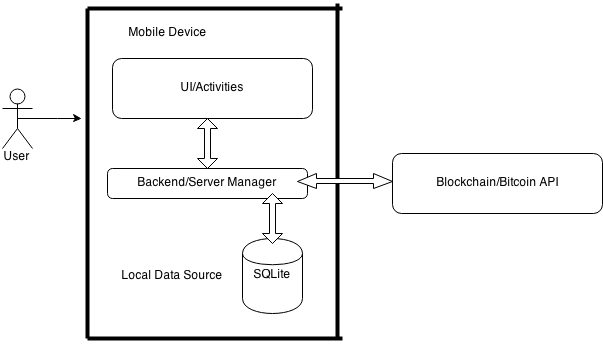
\includegraphics[scale=0.5]{../diagrams/systemArch.png}
	\caption{System Architecture UML}
\end{figure}

%--------Architecture Overview
\textbf{Architecture Overview:}\\
The application will be accessed and stored on an Android phone.  The user will interact with application using touch screen.\\
\begin{itemize}
\item Environment is mobile, can be used anywhere 
\item Users will have existing bitcoin address(es)
\item Main functions consist of storing and organizing bitcoin wallet(s) information and displaying data
\item Input is users bitcoin address(es), output is data organization and customization\\
\end{itemize}

%--------Logical Overview
\textbf{Logical Overview:}\\

\begin{itemize}
\item Utilizing Android OS on mobile phones (minimum Android SDK v4.0 Ice Cream Sandwich), developing in Android SDK framework using JAVA
\item Data storage will be local, utilizing ActiveAndroid ORM
\item Data gathered form bitcoin address(es) using blockchain and bitcoin API
\item IDE will Google's Android Studio\\
\end{itemize}
	
%-------- UI/Activities Description
\textbf{UI/Activities:}\\
\begin{itemize}
\item Will be designed using Android SDK standards in XML mark-up 
\item Purpose provides interaction with end user
\item Interactions include end user input and data binding with back-end/server manager\\
\end{itemize}

%--------- Back-end/Server Description
\textbf{Back-end/Server manager:}\\
\begin{itemize}
\item Will be designed using Android SDK standards in Java
\item Purpose provides interaction between database, blockchain, bitcoin API, and UI/Activities
\item Data binding will occur in this area
\item Interactions include data management, activities controller, and external data management\\
\end{itemize}

%---------- SQLite Description
\textbf{ActiveAndroid ORM:}\\
\begin{itemize}
\item Will be designed using  ActiveAndroid ORM utilizing sql queries and statements 
\item Purpose provides data storage and management for the application
\item Interactions include Back-end/Server communication for queries and storage\\
\end{itemize}

%----------- Blockchain/Bitcoin API Description
\textbf{Blockchain/Bitcoin:}\\
\begin{itemize}
\item Bitcoin interaction in application will be limited to API interaction and blockchain interaction
\item Will not need to be designed. Will be managed by Back-end/Server and BitcoinJ libraries.
\item Purpose is to provide data and information from blockchain and user's existing bitcoin account(s)
\item Interactions will occur with designated API services.\\
\end{itemize}


%------------Class Architecture
\begin{figure}[H]
	\centering
	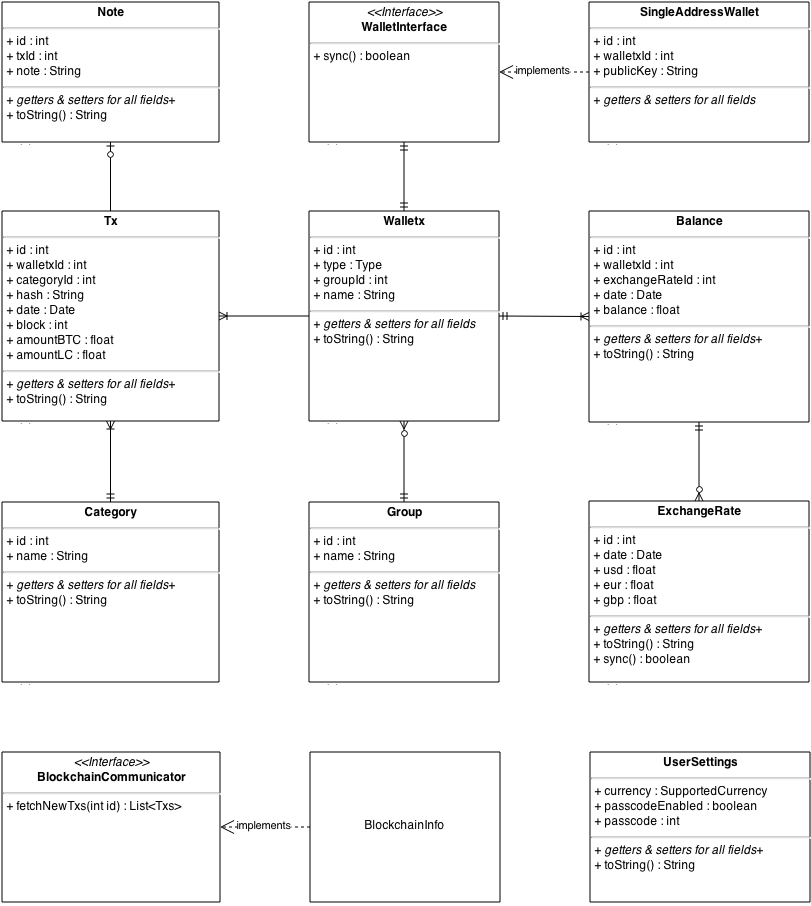
\includegraphics[scale=0.5]{../diagrams/classes_model.png}
	\caption{Class Models}
\end{figure}


\begin{figure}[H]
	\centering
	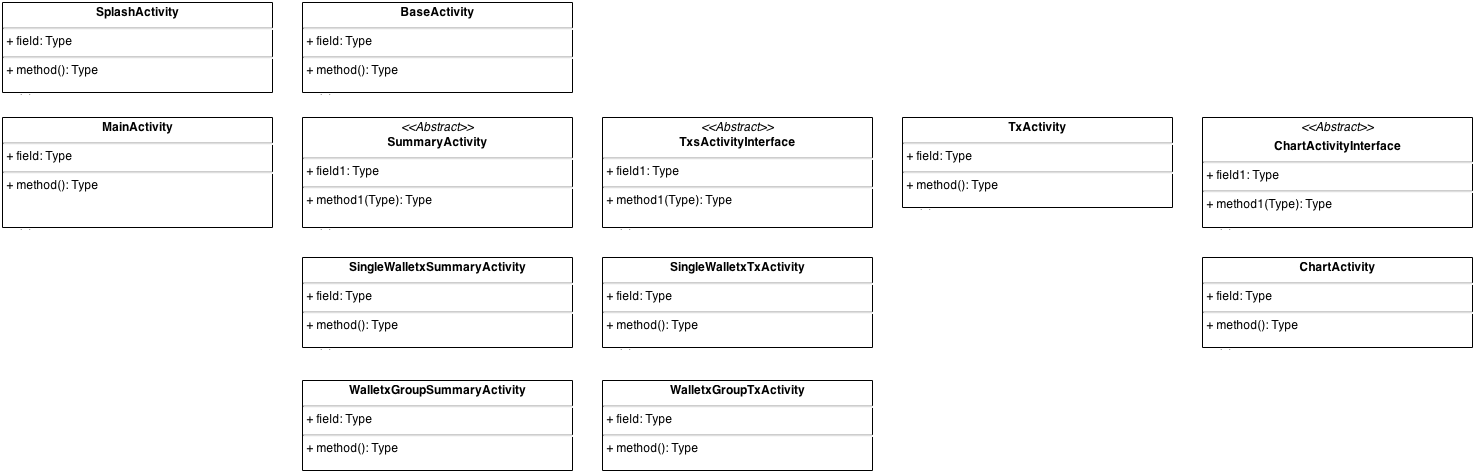
\includegraphics[scale=0.5]{../diagrams/classes_activity.png}
	\caption{Class Activities}
\end{figure}

%------------Database Schema

\begin{figure}[H]
	\centering
	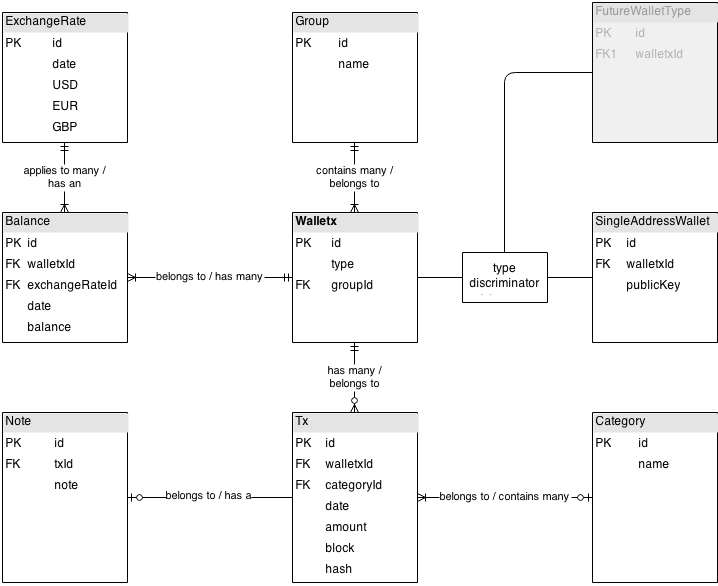
\includegraphics[scale=0.5]{../diagrams/schema.png}
	\caption{Database Schema}
\end{figure}



  \clearpage
\section{System Model}

\begin{figure}[H]
    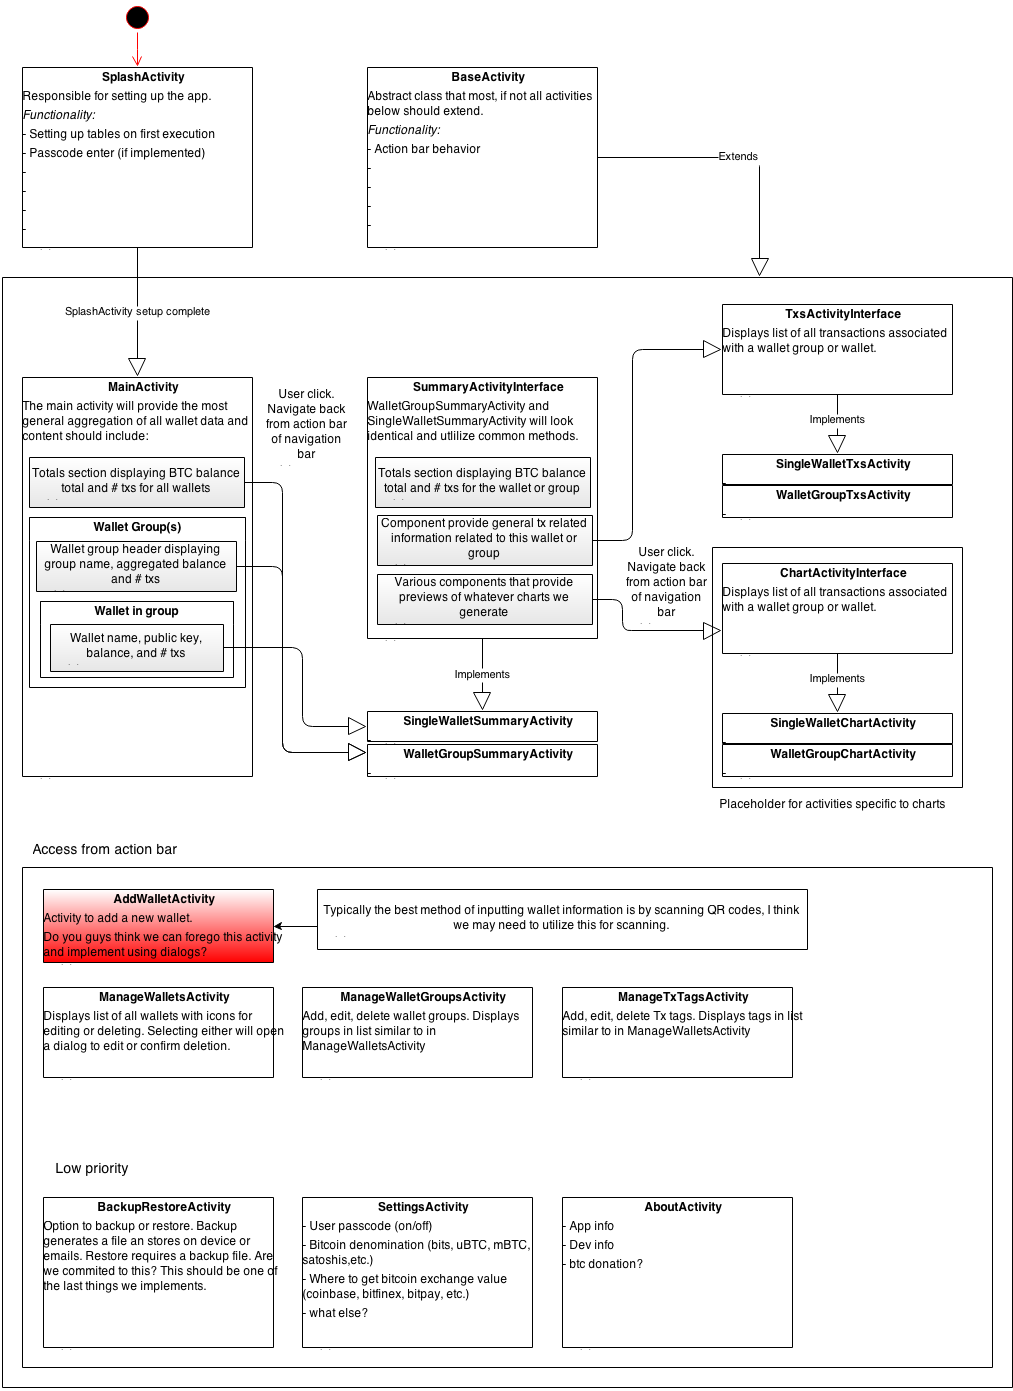
\includegraphics[width=0.9\textwidth]{../diagrams/activities.png}
\end{figure}

  % Change figure labeling to section and #
\renewcommand\thefigure{\thesection.\arabic{figure}}   

\clearpage
\section{Appendices}
  \subsection{Data Dictionary}
    \subsubsection{Actor Descriptions}

    
Identifying actors:\\
\begin{itemize}
  \item Who will supply, use, or remove information from the system?
  \item Who will use the system?
  \item Who is interested in a certain feature or service provided by the system?
  \item Who will support and maintain the system?
  \item What are the system's external resources?
  \item What other systems will need to interact with the system under development?
\end{itemize}

Actors will be the customer/user of the application.  Most interested in our application would be those interested in Bitcoin. Service and maintenance of the system will be performed by the developers(Prestige Worldwide). Systems external resources will be blockchain, SQLite, and other external wallets providing information. (Michael and Brian please confirm external resources of Bitcoin)

  \subsubsection{Use Case Descriptions}

  %-----------------------------------------------
  % Use case 3.1 : Managing User Wallets
  %-----------------------------------------------

  \begin{figure}[H]
    \centering
    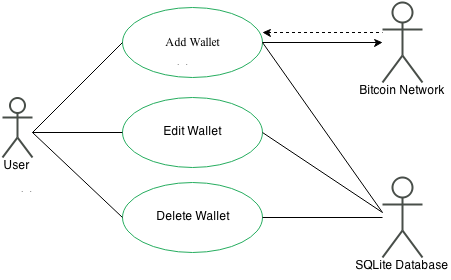
\includegraphics[scale=0.6]{../diagrams/usecase_3_1.png}
    \caption{Managing User Wallets}
  \end{figure}

  % -- Use Case : Add Wallet
  \begin{table}[H]
    \centering
    \resizebox{0.8\columnwidth}{!}{%
    \tabulinesep=1.2mm
    \rowcolors{2}{gray!25}{white}
    \begin{tabu}{| r | X |}
      \rowfont{\color{black}}
      \taburulecolor{black}
      \hline
      \taburowcolors 1{green .. green}
      \multicolumn{2}{|l|}{\textbf{\textsf{WalleTx: Add Wallet}}}\\
      \hline

      \taburowcolors 2{light-gray .. white}
      Actors & User, SQLite Database, Blockchain API\\
      Description & User will add an existing wallet public key to the application to enable mapping of transactions to the wallet public address\\
      Data & public wallet address, transaction hashes, tags associate with transactions\\
      Stimulus & User initiated option\\
      Response & Additional view will open up allowing the user to manual type their wallet address, paste from the clipboard, or scan a qr code. After a valid bitcoin public address is entered the application will contact the Blockchain.info API to pull transaction information putting that information into the database. View will return to the main wallet view.\\
      Comments & \\

      \taburowcolors 1{green .. green}
      \multicolumn{2}{|l|}{\textbf{\textsf{\footnotesize{Figure 7.1}}}}\\
      \hline
    \end{tabu}%
  }
  \end{table}

  % -- Use Case : Modify Wallet
  \begin{table}[H]
    \centering
    \resizebox{0.8\columnwidth}{!}{%
    \tabulinesep=1.2mm
    \rowcolors{2}{gray!25}{white}
    \begin{tabu}{r | X}
      \rowfont{\color{black}}
      \taburulecolor{black}

      \taburowcolors 1{green .. green}
      \multicolumn{2}{l}{\textbf{\textsf{WalleTx: Modify Wallet}}}\\
      \hline

      \taburowcolors 2{light-gray .. white}
      Actors & User, SQLite Database\\
      Description & User will be able to edit the name of the wallet.\\
      Data & Public Wallet Address associated with database entries\\
      Stimulus & User initiated option\\
      Response & View will open allowing the user to change the name of the wallet.\\
      Comments & Changing the wallet address would only serve to change all the underlying transactions, therefore it may be a better idea to only allow adding or removing public wallet addresses to manipulate public wallet address data in the database. Other features not implemented by the Bitcoin blockchain, such as currency pair, wallet nickname, etc. can be modified here.\\
    \end{tabu}%
  }
  \end{table}

  % -- Use Case : Remove Wallet
  \begin{table}[H]
    \tabulinesep=1.2mm
    \centering
    \resizebox{0.8\columnwidth}{!}{%
    \rowcolors{2}{gray!25}{white}
    \begin{tabu}{r | X}
      \rowfont{\color{black}}
      \taburulecolor{black}

      \taburowcolors 1{green .. green}
      \multicolumn{2}{l}{\textbf{\textsf{WalleTx: Remove Wallet}}}\\
      \hline

      \taburowcolors 2{light-gray .. white}
      Actors & User, SQLite Database\\
      Description & User will remove an existing wallet public key from the application and have corresponding data removed from the SQLite database.\\
      Data & public wallet address\\
      Stimulus & User initiated option\\
      Response & Dialog will pop up allowing the user to confirm (possibly have a text input required to continue) and when confirmed the data will be purged from the database.\\
      Comments & \\
    \end{tabu}%
  }
  \end{table}

  %-----------------------------------------------
  % Use case 3.2 : Managing wallet groups
  %-----------------------------------------------
\begin{figure}[H]
    \centering
    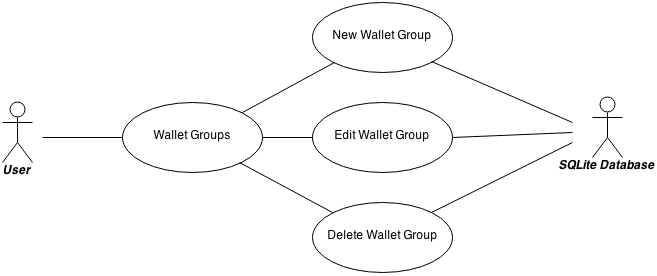
\includegraphics[scale=0.6]{../diagrams/usecase_3_2.png}
    \caption{Managing Wallet Groups}
  \end{figure}
  
  % -- Use Case 3.2 : View all wallet groups 
  \begin{table}[H]
    \tabulinesep=1.2mm
    \centering
    \resizebox{0.8\columnwidth}{!}{%
    \rowcolors{2}{gray!25}{white}
    \begin{tabu}{r | X}
      \rowfont{\color{black}}
      \taburulecolor{black}
      \taburowcolors 1{green .. green}
      \multicolumn{2}{l}{\textbf{\textsf{WalleTx: View all transaction tag categories}}}\\
      \hline
      \taburowcolors 2{light-gray .. white}
      Actors & 
        User, SQLite Database\\
      Description & 
        User is presented with a list view of wallet groups with options to: (1) Add a new wallet group, (2) Edit a wallet group, and (3) Delete a wallet group\\
      Data & 
        Wallet group categories\\
      Stimulus & 
        User initiated option. User selects Wallet Groups from the menu\\
      Response & 
        Application opens CRUDGroupActivity and populates the list view with all the groups in the group table\\
      Comments & 
        This is entry point for user to add, edit and delete wallet groups\\
      \taburowcolors 1{green .. green}
      \multicolumn{2}{|l|}{\textbf{\textsf{\footnotesize{Figure 7.3}}}}\\
      \hline
    \end{tabu}%
  }
  \end{table}

  % -- Use Case 3.2.2 : Add New Wallet Group 
  \begin{table}[H]
    \tabulinesep=1.2mm
    \centering
    \resizebox{0.8\columnwidth}{!}{%
    \rowcolors{2}{gray!25}{white}
    \begin{tabu}{r | X}
      \rowfont{\color{black}}
      \taburulecolor{black}
      \taburowcolors 1{green .. green}
      \multicolumn{2}{l}{\textbf{\textsf{WalleTx: Add wallet group category}}}\\
      \hline
      \taburowcolors 2{light-gray .. white}
      Actors & 
        User, SQLite Database\\
      Description & 
        User adds a new wallet group (by name) to the application\\
      Data & 
        Wallet group name\\
      Stimulus & 
        User initiated option\\
      Response & 
        A dialog will open containing: (1) a text field for entering the new wallet group, (2) a Cancel button, (3) and an Add button. If Add is selected, user entered wallet group name is inserted into the Wallet Group table and user is returned to the CRUDGroupActivity. If cancel is selected, user is returned to the CRUDGroupActivity.\\
      Comments & 
        Response should validate for empty wallet group name. CRUDGroupActivity UI must be updated upon successful insertion of a new tag category\\
      \taburowcolors 1{green .. green}
      \multicolumn{2}{|l|}{\textbf{\textsf{\footnotesize{Figure 7.3}}}}\\
      \hline
    \end{tabu}%
  }
  \end{table}

  % -- Use Case 3.2.3 : Edit Wallet Group
  \begin{table}[H]
    \tabulinesep=1.2mm
    \centering
    \resizebox{0.8\columnwidth}{!}{%
    \rowcolors{2}{gray!25}{white}
    \begin{tabu}{r | X}
      \rowfont{\color{black}}
      \taburulecolor{black}
      \taburowcolors 1{green .. green}
      \multicolumn{2}{l}{\textbf{\textsf{WalleTx: Edit wallet group category}}}\\
      \hline
      \taburowcolors 2{light-gray .. white}
      Actors & 
        User, SQLite Database\\
      Description & 
        User edits an existing wallet group\\
      Data & 
        Wallet group name\\
      Stimulus & 
        User initiated option. User selects edit button from wallet group view.\\
      Response & 
        A dialog will open containing: (1) an edit text field for updating wallet group, (2) a Cancel button, (3) and an Edit button. If Edit is selected, the wallet group is updated in the Wallet Group table and user is returned to the CRUDGroupActivity. If cancel is selected, user is returned to the CRUDGroupActivity.\\
      Comments & 
        Response should validate for empty wallet group name. CRUDGroupActivity UI must be updated upon successful update of a tag category\\
      \taburowcolors 1{green .. green}
      \multicolumn{2}{|l|}{\textbf{\textsf{\footnotesize{Figure 7.3}}}}\\
      \hline
    \end{tabu}%
  }
  \end{table}

  % -- Use Case 3.2.4 : Delete wallet group
  \begin{table}[H]
    \tabulinesep=1.2mm
    \centering
    \resizebox{0.8\columnwidth}{!}{%
    \rowcolors{2}{gray!25}{white}
    \begin{tabu}{r | X}
      \rowfont{\color{black}}
      \taburulecolor{black}
      \taburowcolors 1{green .. green}
      \multicolumn{2}{l}{\textbf{\textsf{WalleTx: Delete Wallet Group}}}\\
      \hline
      \taburowcolors 2{light-gray .. white}
      Actors & 
        User, SQLite Database\\
      Description & 
        User deletes an existing wallet group\\
      Data & 
        Wallet group name\\
      Stimulus & 
        User initiated option. User selects delete button from wallet group list view.\\
      Response & 
        A dialog will open confirming if user wishes to delete the wallet group. If confirmed, the wallet group must be removed then reassign all wallets associated with deleted group to the default group and then removed from the Wallet Group table. User is then returned to the CRUDGroupActivity.\\
      Comments & 
        CRUDGroupActivity UI must be updated upon successful update of the wallet groups\\
      \taburowcolors 1{green .. green}
      \multicolumn{2}{|l|}{\textbf{\textsf{\footnotesize{Figure 7.3}}}}\\
      \hline
    \end{tabu}%
  }
  \end{table}
  
  
  %-----------------------------------------------
  % Use case 3.3 : Managing tx tag categories
  %-----------------------------------------------

  \begin{figure}[H]
    \centering
    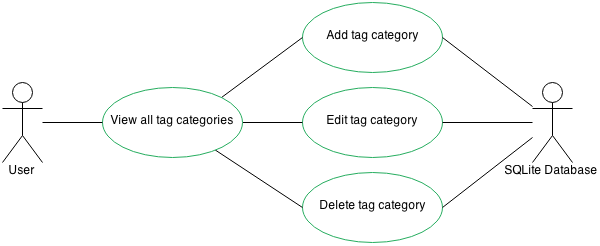
\includegraphics[scale=0.6]{../diagrams/usecase_3_3.png}
    \caption{Managing Transaction Tag Categories}
  \end{figure}

  % -- Use Case 3.3 : View all tag categories
  \begin{table}[H]
    \tabulinesep=1.2mm
    \centering
    \resizebox{0.8\columnwidth}{!}{%
    \rowcolors{2}{gray!25}{white}
    \begin{tabu}{r | X}
      \rowfont{\color{black}}
      \taburulecolor{black}
      \taburowcolors 1{green .. green}
      \multicolumn{2}{l}{\textbf{\textsf{WalleTx: View all transaction tag categories}}}\\
      \hline
      \taburowcolors 2{light-gray .. white}
      Actors & 
        User, SQLite Database\\
      Description & 
        User is presented with a list view of all tags with options to: (1) Add a new tag, (2) Edit a tag, and (3) Delete a tag\\
      Data & 
        Tags categories\\
      Stimulus & 
        User initiated option. User selects Tx Tags from the menu\\
      Response & 
        Application opens CRUDTagsActivity and populates the list view with all tags in the Tag table\\
      Comments & 
        This is entry point for user to add, edit and delete tags\\
      \taburowcolors 1{green .. green}
      \multicolumn{2}{|l|}{\textbf{\textsf{\footnotesize{Figure 7.3}}}}\\
      \hline
    \end{tabu}%
  }
  \end{table}

  % -- Use Case 3.3.1 : Add tag category
  \begin{table}[H]
    \tabulinesep=1.2mm
    \centering
    \resizebox{0.8\columnwidth}{!}{%
    \rowcolors{2}{gray!25}{white}
    \begin{tabu}{r | X}
      \rowfont{\color{black}}
      \taburulecolor{black}
      \taburowcolors 1{green .. green}
      \multicolumn{2}{l}{\textbf{\textsf{WalleTx: Add transaction tag category}}}\\
      \hline
      \taburowcolors 2{light-gray .. white}
      Actors & 
        User, SQLite Database\\
      Description & 
        User adds a new tag category (by name) to the application\\
      Data & 
        Tag category name\\
      Stimulus & 
        User initiated option\\
      Response & 
        A dialog will open containing: (1) a text field for entering the new tag category, (2) a Cancel button, (3) and an Add button. If Add is selected, user entered tag category is inserted into the Tag table and user is returned to the CRUDTagsActivity. If cancel is selected, user is returned to the CRUDTagsActivity.\\
      Comments & 
        Response should validate for empty tag name. CRUDTagsActivity UI must be updated upon successful insertion of a new tag category\\
      \taburowcolors 1{green .. green}
      \multicolumn{2}{|l|}{\textbf{\textsf{\footnotesize{Figure 7.3}}}}\\
      \hline
    \end{tabu}%
  }
  \end{table}

  % -- Use Case 3.3.2 : Edit tag category
  \begin{table}[H]
    \tabulinesep=1.2mm
    \centering
    \resizebox{0.8\columnwidth}{!}{%
    \rowcolors{2}{gray!25}{white}
    \begin{tabu}{r | X}
      \rowfont{\color{black}}
      \taburulecolor{black}
      \taburowcolors 1{green .. green}
      \multicolumn{2}{l}{\textbf{\textsf{WalleTx: Edit transaction tag category}}}\\
      \hline
      \taburowcolors 2{light-gray .. white}
      Actors & 
        User, SQLite Database\\
      Description & 
        User edits an existing tag category\\
      Data & 
        Tag category name\\
      Stimulus & 
        User initiated option. User selects edit button from tags list view.\\
      Response & 
        A dialog will open containing: (1) an edit text field for updating tag category, (2) a Cancel button, (3) and an Edit button. If Edit is selected, the tag is updated in the Tag table and user is returned to the CRUDTagsActivity. If cancel is selected, user is returned to the CRUDTagsActivity.\\
      Comments & 
        Response should validate for empty tag name. CRUDTagsActivity UI must be updated upon successful update of a tag category\\
      \taburowcolors 1{green .. green}
      \multicolumn{2}{|l|}{\textbf{\textsf{\footnotesize{Figure 7.3}}}}\\
      \hline
    \end{tabu}%
  }
  \end{table}

  % -- Use Case 3.3.3 : Delete tag category
  \begin{table}[H]
    \tabulinesep=1.2mm
    \centering
    \resizebox{0.8\columnwidth}{!}{%
    \rowcolors{2}{gray!25}{white}
    \begin{tabu}{r | X}
      \rowfont{\color{black}}
      \taburulecolor{black}
      \taburowcolors 1{green .. green}
      \multicolumn{2}{l}{\textbf{\textsf{WalleTx: Delete transaction tag category}}}\\
      \hline
      \taburowcolors 2{light-gray .. white}
      Actors & 
        User, SQLite Database\\
      Description & 
        User deletes an existing tag category\\
      Data & 
        Tag category name\\
      Stimulus & 
        User initiated option. User selects delete button from tags list view.\\
      Response & 
        A dialog will open confirming if user wishes to delete the tag. If confirmed, the tag must be removed from any transactions onto which it is applied and then removed from the Tags table. User is then returned to the CRUDTagsActivity.\\
      Comments & 
        CRUDTagsActivity UI must be updated upon successful update of a tag category\\
      \taburowcolors 1{green .. green}
      \multicolumn{2}{|l|}{\textbf{\textsf{\footnotesize{Figure 7.3}}}}\\
      \hline
    \end{tabu}%
  }
  \end{table}

  %-----------------------------------------------
  % Use case 3.4 : Tagging transactions
  %-----------------------------------------------








    \begin{figure}[ht]
      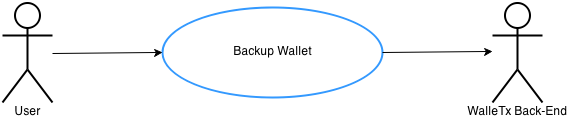
\includegraphics[width=1.0\textwidth]{./section7/diagrams/use-case-backup.png}
    \end{figure}

\begin{table}[H]
  \tabulinesep=1.2mm
      \rowcolors{2}{gray!25}{white}
      \begin{tabu}{r | X}
        \rowfont{\color{black}}
        \taburulecolor{white}
        \taburowcolors 2{light-gray .. white}
        \multicolumn{2}{l}{\textbf{\textsf{WalleTx: Backup Data}}}\\
        \hline
        \textsf{Actors} & User\\
        Description & A user will be able to backup all wallet information, transaction hashes, and tags associate with those transactions to an XML or JSON file.\\
        Data & public wallet identification, transaction hashes, tags associate with transactions\\
        Stimulus & User initiates a data backup\\
        Response & Dialog box will confirm backup\\
        Comments & Is there any additional data that needs to be backed up? Where will the database backup be stored?\\
      \end{tabu}
    \end{table}


Identifying use cases:\\
\begin{itemize}
\item What are the goals that the actor will attempt to accomplish with the system?
\item What are the primary tasks that the actor wants the system to perform?
\item Will the actor create, store, change, remove, or read data in the system?
\item Will the actor need to inform the system about sudden external changes?
\item Does the actor need to be informed about certain occurrences, such as unavailability of a network resource, in the system?
\item Will the actor perform a system startup or shutdown?
\end{itemize}

Use cases will be outlined in diagrams provided.\\ 

The primary task of the customer/user will be to interact with the application.  Their main purpose will be to monitor their bitcoin currency from multiple wallets and tag transactions to better organize all transactions.  The actor will have the ability to add and remove wallets/add and remove tags pertaining to transactions. The actor can observe aggregate information in the form of graphs, charts, etc.  The actor will be alerted to certain trigger events. (updated wallet info, specific transactions, etc).  The actor has the ability to close and open application in running OS and also has the ability to completely remove the application from existing OS. \\
	
	
    \subsubsection{Class Descriptions}
      \begin{figure}[H]
%        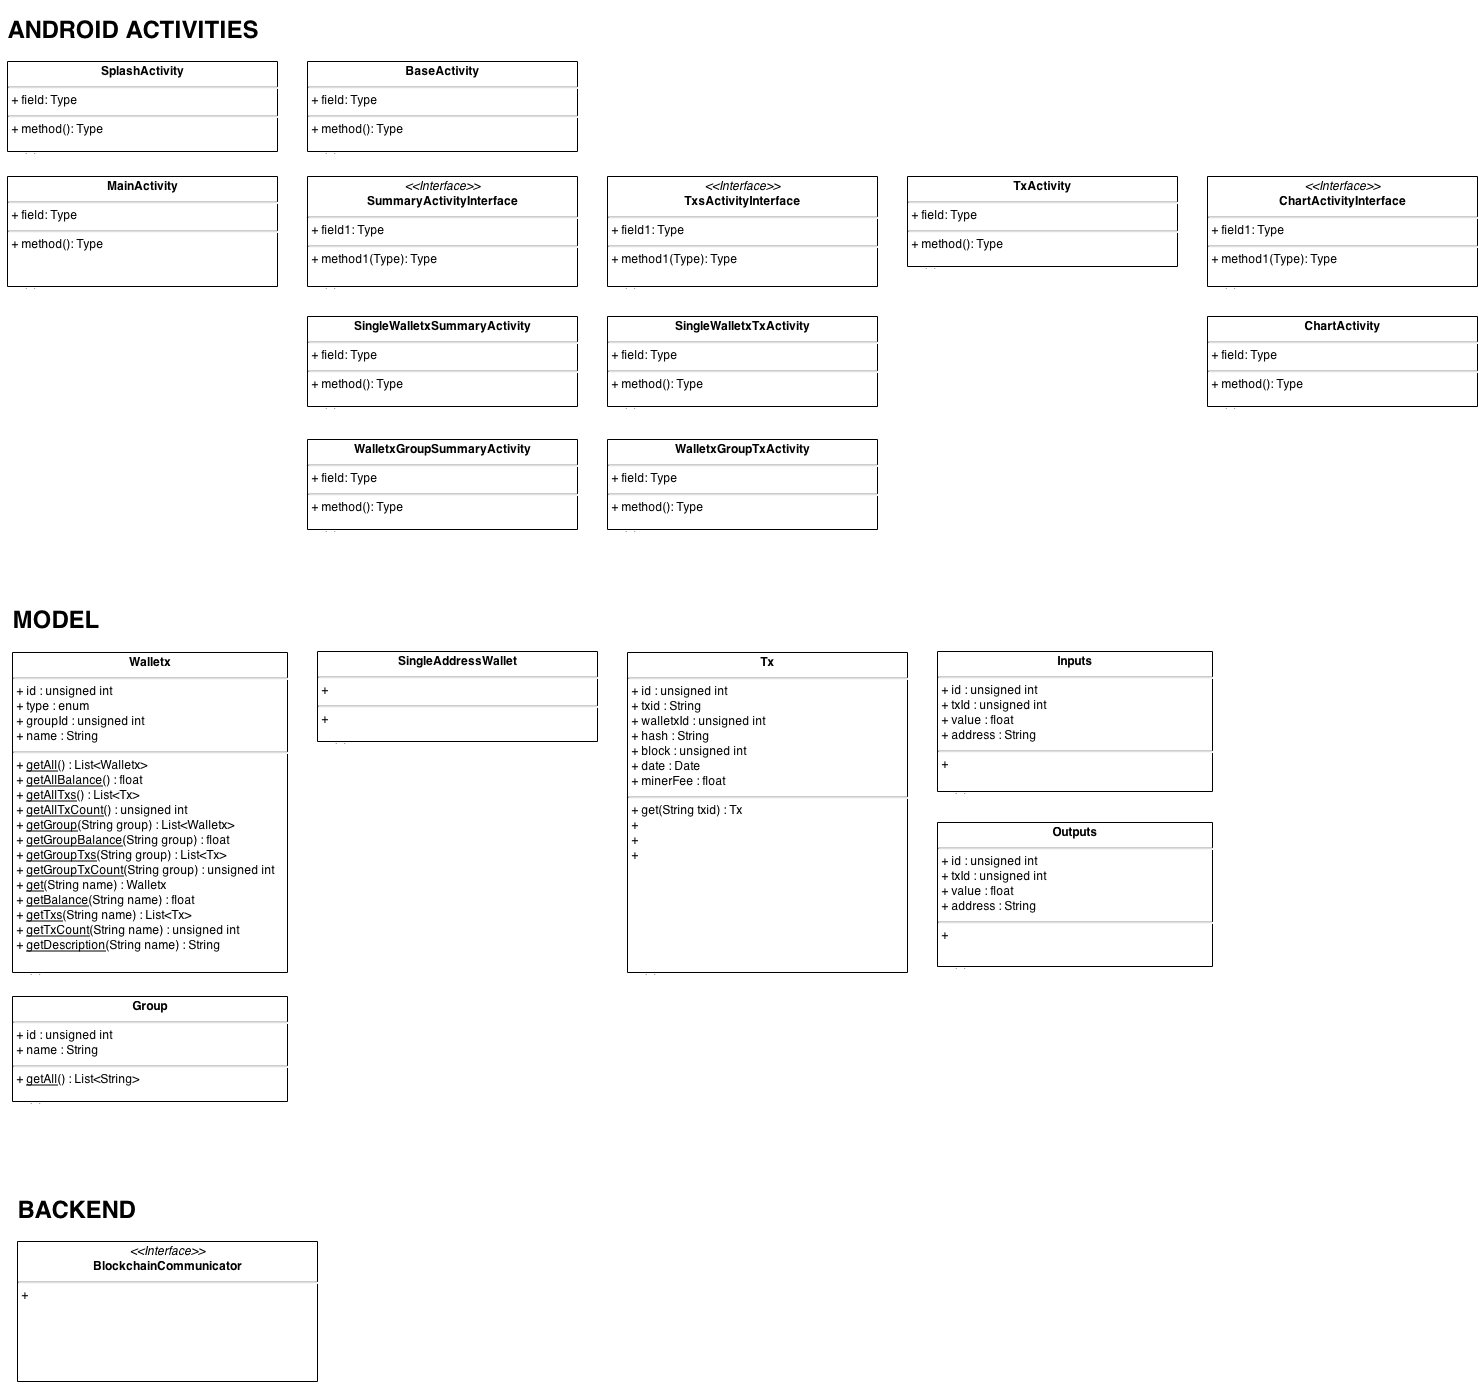
\includegraphics[width=1.0\textwidth]{../diagrams/classes.png}
      \end{figure}

    \subsubsection{Attribute Descriptions}
  \subsection{Raw Use Case Point Analysis}
    \subsubsection{Actor Summary Table}
    \begin{table}[H]
      \begin{tabularx}{\textwidth}{r | X}
        Actors                       & Summary\\
        \hline
        Customer/End User            & This actor will be the end user.  They will interact with WalleTx,  providing it with wallet information, tagging transactions, and viewing  aggrated wallet information\\
        Development Team/Maintenance & This actor will be interacting via the support and maintance of the  application.  They will maintain DB orginzation, revision handling, and  overall maintaince of the application\\
        External Bitcoin Wallets     & External Bitcoin Wallets will be providing our application with vital  information.  All external wallets' totals and transactions will  aggreated in WalleTx.\\
        SQLite Database              & This actor is a database stored on each end user's phone. This will  contain data from wallets, transactions, and display information.  It  will interact soley with the application via code.\\
        Bitcoin Blockchain           & The bitcoin blocktrain will provide transaction specific data for all  included wallets. This actor will interact with the application via  database backend.\\
      \end{tabularx}
    \end{table}

    \subsubsection{Use Case Summary Table}

    \subsubsection{Screens and Reports with Navigation Matrix}
  \subsection{Other Appendices}


 \end{document}
